% Generated by Sphinx.
\def\sphinxdocclass{report}
\documentclass[letterpaper,10pt,english]{sphinxmanual}
\usepackage[utf8]{inputenc}
\DeclareUnicodeCharacter{00A0}{\nobreakspace}
\usepackage{cmap}
\usepackage[T1]{fontenc}
\usepackage{babel}
\usepackage{times}
\usepackage[Bjarne]{fncychap}
\usepackage{longtable}
\usepackage{sphinx}
\usepackage{multirow}

\addto\captionsenglish{\renewcommand{\figurename}{Fig. }}
\addto\captionsenglish{\renewcommand{\tablename}{Table }}
\floatname{literal-block}{Listing }



\title{fastFM Documentation}
\date{July 03, 2015}
\release{0.1.0}
\author{Immanuel Bayer}
\newcommand{\sphinxlogo}{}
\renewcommand{\releasename}{Release}
\makeindex

\makeatletter
\def\PYG@reset{\let\PYG@it=\relax \let\PYG@bf=\relax%
    \let\PYG@ul=\relax \let\PYG@tc=\relax%
    \let\PYG@bc=\relax \let\PYG@ff=\relax}
\def\PYG@tok#1{\csname PYG@tok@#1\endcsname}
\def\PYG@toks#1+{\ifx\relax#1\empty\else%
    \PYG@tok{#1}\expandafter\PYG@toks\fi}
\def\PYG@do#1{\PYG@bc{\PYG@tc{\PYG@ul{%
    \PYG@it{\PYG@bf{\PYG@ff{#1}}}}}}}
\def\PYG#1#2{\PYG@reset\PYG@toks#1+\relax+\PYG@do{#2}}

\expandafter\def\csname PYG@tok@gd\endcsname{\def\PYG@tc##1{\textcolor[rgb]{0.63,0.00,0.00}{##1}}}
\expandafter\def\csname PYG@tok@gu\endcsname{\let\PYG@bf=\textbf\def\PYG@tc##1{\textcolor[rgb]{0.50,0.00,0.50}{##1}}}
\expandafter\def\csname PYG@tok@gt\endcsname{\def\PYG@tc##1{\textcolor[rgb]{0.00,0.27,0.87}{##1}}}
\expandafter\def\csname PYG@tok@gs\endcsname{\let\PYG@bf=\textbf}
\expandafter\def\csname PYG@tok@gr\endcsname{\def\PYG@tc##1{\textcolor[rgb]{1.00,0.00,0.00}{##1}}}
\expandafter\def\csname PYG@tok@cm\endcsname{\def\PYG@tc##1{\textcolor[rgb]{0.53,0.53,0.53}{##1}}}
\expandafter\def\csname PYG@tok@vg\endcsname{\let\PYG@bf=\textbf\def\PYG@tc##1{\textcolor[rgb]{0.87,0.47,0.00}{##1}}}
\expandafter\def\csname PYG@tok@m\endcsname{\let\PYG@bf=\textbf\def\PYG@tc##1{\textcolor[rgb]{0.40,0.00,0.93}{##1}}}
\expandafter\def\csname PYG@tok@mh\endcsname{\let\PYG@bf=\textbf\def\PYG@tc##1{\textcolor[rgb]{0.00,0.33,0.53}{##1}}}
\expandafter\def\csname PYG@tok@cs\endcsname{\let\PYG@bf=\textbf\def\PYG@tc##1{\textcolor[rgb]{0.80,0.00,0.00}{##1}}}
\expandafter\def\csname PYG@tok@ge\endcsname{\let\PYG@it=\textit}
\expandafter\def\csname PYG@tok@vc\endcsname{\def\PYG@tc##1{\textcolor[rgb]{0.20,0.40,0.60}{##1}}}
\expandafter\def\csname PYG@tok@il\endcsname{\let\PYG@bf=\textbf\def\PYG@tc##1{\textcolor[rgb]{0.00,0.00,0.87}{##1}}}
\expandafter\def\csname PYG@tok@go\endcsname{\def\PYG@tc##1{\textcolor[rgb]{0.53,0.53,0.53}{##1}}}
\expandafter\def\csname PYG@tok@cp\endcsname{\def\PYG@tc##1{\textcolor[rgb]{0.33,0.47,0.60}{##1}}}
\expandafter\def\csname PYG@tok@gi\endcsname{\def\PYG@tc##1{\textcolor[rgb]{0.00,0.63,0.00}{##1}}}
\expandafter\def\csname PYG@tok@gh\endcsname{\let\PYG@bf=\textbf\def\PYG@tc##1{\textcolor[rgb]{0.00,0.00,0.50}{##1}}}
\expandafter\def\csname PYG@tok@ni\endcsname{\let\PYG@bf=\textbf\def\PYG@tc##1{\textcolor[rgb]{0.53,0.00,0.00}{##1}}}
\expandafter\def\csname PYG@tok@nl\endcsname{\let\PYG@bf=\textbf\def\PYG@tc##1{\textcolor[rgb]{0.60,0.47,0.00}{##1}}}
\expandafter\def\csname PYG@tok@nn\endcsname{\let\PYG@bf=\textbf\def\PYG@tc##1{\textcolor[rgb]{0.05,0.52,0.71}{##1}}}
\expandafter\def\csname PYG@tok@no\endcsname{\let\PYG@bf=\textbf\def\PYG@tc##1{\textcolor[rgb]{0.00,0.20,0.40}{##1}}}
\expandafter\def\csname PYG@tok@na\endcsname{\def\PYG@tc##1{\textcolor[rgb]{0.00,0.00,0.80}{##1}}}
\expandafter\def\csname PYG@tok@nb\endcsname{\def\PYG@tc##1{\textcolor[rgb]{0.00,0.44,0.13}{##1}}}
\expandafter\def\csname PYG@tok@nc\endcsname{\let\PYG@bf=\textbf\def\PYG@tc##1{\textcolor[rgb]{0.73,0.00,0.40}{##1}}}
\expandafter\def\csname PYG@tok@nd\endcsname{\let\PYG@bf=\textbf\def\PYG@tc##1{\textcolor[rgb]{0.33,0.33,0.33}{##1}}}
\expandafter\def\csname PYG@tok@ne\endcsname{\let\PYG@bf=\textbf\def\PYG@tc##1{\textcolor[rgb]{1.00,0.00,0.00}{##1}}}
\expandafter\def\csname PYG@tok@nf\endcsname{\let\PYG@bf=\textbf\def\PYG@tc##1{\textcolor[rgb]{0.00,0.40,0.73}{##1}}}
\expandafter\def\csname PYG@tok@si\endcsname{\def\PYG@bc##1{\setlength{\fboxsep}{0pt}\colorbox[rgb]{0.93,0.93,0.93}{\strut ##1}}}
\expandafter\def\csname PYG@tok@s2\endcsname{\def\PYG@bc##1{\setlength{\fboxsep}{0pt}\colorbox[rgb]{1.00,0.94,0.94}{\strut ##1}}}
\expandafter\def\csname PYG@tok@vi\endcsname{\def\PYG@tc##1{\textcolor[rgb]{0.20,0.20,0.73}{##1}}}
\expandafter\def\csname PYG@tok@nt\endcsname{\def\PYG@tc##1{\textcolor[rgb]{0.00,0.47,0.00}{##1}}}
\expandafter\def\csname PYG@tok@nv\endcsname{\def\PYG@tc##1{\textcolor[rgb]{0.60,0.40,0.20}{##1}}}
\expandafter\def\csname PYG@tok@s1\endcsname{\def\PYG@bc##1{\setlength{\fboxsep}{0pt}\colorbox[rgb]{1.00,0.94,0.94}{\strut ##1}}}
\expandafter\def\csname PYG@tok@gp\endcsname{\let\PYG@bf=\textbf\def\PYG@tc##1{\textcolor[rgb]{0.78,0.36,0.04}{##1}}}
\expandafter\def\csname PYG@tok@sh\endcsname{\def\PYG@bc##1{\setlength{\fboxsep}{0pt}\colorbox[rgb]{1.00,0.94,0.94}{\strut ##1}}}
\expandafter\def\csname PYG@tok@ow\endcsname{\let\PYG@bf=\textbf\def\PYG@tc##1{\textcolor[rgb]{0.00,0.00,0.00}{##1}}}
\expandafter\def\csname PYG@tok@sx\endcsname{\def\PYG@tc##1{\textcolor[rgb]{0.87,0.13,0.00}{##1}}\def\PYG@bc##1{\setlength{\fboxsep}{0pt}\colorbox[rgb]{1.00,0.94,0.94}{\strut ##1}}}
\expandafter\def\csname PYG@tok@bp\endcsname{\def\PYG@tc##1{\textcolor[rgb]{0.00,0.44,0.13}{##1}}}
\expandafter\def\csname PYG@tok@c1\endcsname{\def\PYG@tc##1{\textcolor[rgb]{0.53,0.53,0.53}{##1}}}
\expandafter\def\csname PYG@tok@kc\endcsname{\let\PYG@bf=\textbf\def\PYG@tc##1{\textcolor[rgb]{0.00,0.53,0.00}{##1}}}
\expandafter\def\csname PYG@tok@c\endcsname{\def\PYG@tc##1{\textcolor[rgb]{0.53,0.53,0.53}{##1}}}
\expandafter\def\csname PYG@tok@mf\endcsname{\let\PYG@bf=\textbf\def\PYG@tc##1{\textcolor[rgb]{0.40,0.00,0.93}{##1}}}
\expandafter\def\csname PYG@tok@err\endcsname{\def\PYG@tc##1{\textcolor[rgb]{1.00,0.00,0.00}{##1}}\def\PYG@bc##1{\setlength{\fboxsep}{0pt}\colorbox[rgb]{1.00,0.67,0.67}{\strut ##1}}}
\expandafter\def\csname PYG@tok@mb\endcsname{\let\PYG@bf=\textbf\def\PYG@tc##1{\textcolor[rgb]{0.40,0.00,0.93}{##1}}}
\expandafter\def\csname PYG@tok@ss\endcsname{\def\PYG@tc##1{\textcolor[rgb]{0.67,0.40,0.00}{##1}}}
\expandafter\def\csname PYG@tok@sr\endcsname{\def\PYG@tc##1{\textcolor[rgb]{0.00,0.00,0.00}{##1}}\def\PYG@bc##1{\setlength{\fboxsep}{0pt}\colorbox[rgb]{1.00,0.94,1.00}{\strut ##1}}}
\expandafter\def\csname PYG@tok@mo\endcsname{\let\PYG@bf=\textbf\def\PYG@tc##1{\textcolor[rgb]{0.27,0.00,0.93}{##1}}}
\expandafter\def\csname PYG@tok@kd\endcsname{\let\PYG@bf=\textbf\def\PYG@tc##1{\textcolor[rgb]{0.00,0.53,0.00}{##1}}}
\expandafter\def\csname PYG@tok@mi\endcsname{\let\PYG@bf=\textbf\def\PYG@tc##1{\textcolor[rgb]{0.00,0.00,0.87}{##1}}}
\expandafter\def\csname PYG@tok@kn\endcsname{\let\PYG@bf=\textbf\def\PYG@tc##1{\textcolor[rgb]{0.00,0.53,0.00}{##1}}}
\expandafter\def\csname PYG@tok@o\endcsname{\def\PYG@tc##1{\textcolor[rgb]{0.20,0.20,0.20}{##1}}}
\expandafter\def\csname PYG@tok@kr\endcsname{\let\PYG@bf=\textbf\def\PYG@tc##1{\textcolor[rgb]{0.00,0.53,0.00}{##1}}}
\expandafter\def\csname PYG@tok@s\endcsname{\def\PYG@bc##1{\setlength{\fboxsep}{0pt}\colorbox[rgb]{1.00,0.94,0.94}{\strut ##1}}}
\expandafter\def\csname PYG@tok@kp\endcsname{\let\PYG@bf=\textbf\def\PYG@tc##1{\textcolor[rgb]{0.00,0.20,0.53}{##1}}}
\expandafter\def\csname PYG@tok@w\endcsname{\def\PYG@tc##1{\textcolor[rgb]{0.73,0.73,0.73}{##1}}}
\expandafter\def\csname PYG@tok@kt\endcsname{\let\PYG@bf=\textbf\def\PYG@tc##1{\textcolor[rgb]{0.20,0.20,0.60}{##1}}}
\expandafter\def\csname PYG@tok@sc\endcsname{\def\PYG@tc##1{\textcolor[rgb]{0.00,0.27,0.87}{##1}}}
\expandafter\def\csname PYG@tok@sb\endcsname{\def\PYG@bc##1{\setlength{\fboxsep}{0pt}\colorbox[rgb]{1.00,0.94,0.94}{\strut ##1}}}
\expandafter\def\csname PYG@tok@k\endcsname{\let\PYG@bf=\textbf\def\PYG@tc##1{\textcolor[rgb]{0.00,0.53,0.00}{##1}}}
\expandafter\def\csname PYG@tok@se\endcsname{\let\PYG@bf=\textbf\def\PYG@tc##1{\textcolor[rgb]{0.40,0.40,0.40}{##1}}\def\PYG@bc##1{\setlength{\fboxsep}{0pt}\colorbox[rgb]{1.00,0.94,0.94}{\strut ##1}}}
\expandafter\def\csname PYG@tok@sd\endcsname{\def\PYG@tc##1{\textcolor[rgb]{0.87,0.27,0.13}{##1}}}

\def\PYGZbs{\char`\\}
\def\PYGZus{\char`\_}
\def\PYGZob{\char`\{}
\def\PYGZcb{\char`\}}
\def\PYGZca{\char`\^}
\def\PYGZam{\char`\&}
\def\PYGZlt{\char`\<}
\def\PYGZgt{\char`\>}
\def\PYGZsh{\char`\#}
\def\PYGZpc{\char`\%}
\def\PYGZdl{\char`\$}
\def\PYGZhy{\char`\-}
\def\PYGZsq{\char`\'}
\def\PYGZdq{\char`\"}
\def\PYGZti{\char`\~}
% for compatibility with earlier versions
\def\PYGZat{@}
\def\PYGZlb{[}
\def\PYGZrb{]}
\makeatother

\renewcommand\PYGZsq{\textquotesingle}

\begin{document}

\maketitle
\tableofcontents
\phantomsection\label{index::doc}



\chapter{Tutorials}
\label{tutorial:tutorials}\label{tutorial::doc}\label{tutorial:welcome-to-fastfm-s-documentation}
The following sections show how to use different features of the fastFM
library. The focus in on how to use the library and not on the Factorization
Machine model. I recommend to read {[}TIST2012{]} for examples that show how FM's
can emulate and extend many matrix factorization model through feature engineering.


\section{Regression with ALS Solver}
\label{tutorial:regression-with-als-solver}
We first set up a small toy dataset for a simple regression problem. Please
refere to {[}SIGIR2011{]} for background information on the implemented ALS solver.

\begin{Verbatim}[commandchars=\\\{\}]
\PYG{k+kn}{from} \PYG{n+nn}{fastFM.datasets} \PYG{k+kn}{import} \PYG{n}{make\PYGZus{}user\PYGZus{}item\PYGZus{}regression}
\PYG{k+kn}{from} \PYG{n+nn}{sklearn.cross\PYGZus{}validation} \PYG{k+kn}{import} \PYG{n}{train\PYGZus{}test\PYGZus{}split}

\PYG{c}{\PYGZsh{} This sets up a small test dataset.}
\PYG{n}{X}\PYG{p}{,} \PYG{n}{y}\PYG{p}{,} \PYG{n}{\PYGZus{}} \PYG{o}{=} \PYG{n}{make\PYGZus{}user\PYGZus{}item\PYGZus{}regression}\PYG{p}{(}\PYG{n}{label\PYGZus{}stdev}\PYG{o}{=}\PYG{o}{.}\PYG{l+m+mi}{4}\PYG{p}{)}
\PYG{n}{X\PYGZus{}train}\PYG{p}{,} \PYG{n}{X\PYGZus{}test}\PYG{p}{,} \PYG{n}{y\PYGZus{}train}\PYG{p}{,} \PYG{n}{y\PYGZus{}test} \PYG{o}{=} \PYG{n}{train\PYGZus{}test\PYGZus{}split}\PYG{p}{(}\PYG{n}{X}\PYG{p}{,} \PYG{n}{y}\PYG{p}{)}
\end{Verbatim}

The number of iterations \emph{n\_iter}, the standart derivation \emph{init\_stdev} for The
random initization and the number of hiden variables \emph{rank} per feature have
to be specified for each solver and task. The ALS solver requires us also to
set the regularization for the first \emph{l2\_reg\_w} and second order \emph{l2\_reg\_V} interactions.

\begin{Verbatim}[commandchars=\\\{\}]
\PYG{k+kn}{from} \PYG{n+nn}{fastFM} \PYG{k+kn}{import} \PYG{n}{als}
\PYG{n}{fm} \PYG{o}{=} \PYG{n}{als}\PYG{o}{.}\PYG{n}{FMRegression}\PYG{p}{(}\PYG{n}{n\PYGZus{}iter}\PYG{o}{=}\PYG{l+m+mi}{1000}\PYG{p}{,} \PYG{n}{init\PYGZus{}stdev}\PYG{o}{=}\PYG{l+m+mf}{0.1}\PYG{p}{,} \PYG{n}{rank}\PYG{o}{=}\PYG{l+m+mi}{2}\PYG{p}{,} \PYG{n}{l2\PYGZus{}reg\PYGZus{}w}\PYG{o}{=}\PYG{l+m+mf}{0.1}\PYG{p}{,} \PYG{n}{l2\PYGZus{}reg\PYGZus{}V}\PYG{o}{=}\PYG{l+m+mf}{0.5}\PYG{p}{)}
\PYG{n}{fm}\PYG{o}{.}\PYG{n}{fit}\PYG{p}{(}\PYG{n}{X\PYGZus{}train}\PYG{p}{,} \PYG{n}{y\PYGZus{}train}\PYG{p}{)}
\PYG{n}{y\PYGZus{}pred} \PYG{o}{=} \PYG{n}{fm}\PYG{o}{.}\PYG{n}{predict}\PYG{p}{(}\PYG{n}{X\PYGZus{}test}\PYG{p}{)}
\end{Verbatim}

We can easely evaluate our model using the scikit-learn library.

\begin{Verbatim}[commandchars=\\\{\}]
\PYG{k+kn}{from} \PYG{n+nn}{sklearn.metrics} \PYG{k+kn}{import} \PYG{n}{mean\PYGZus{}squared\PYGZus{}error}
\PYG{l+s}{\PYGZsq{}}\PYG{l+s}{mse:}\PYG{l+s}{\PYGZsq{}}\PYG{p}{,} \PYG{n}{mean\PYGZus{}squared\PYGZus{}error}\PYG{p}{(}\PYG{n}{y\PYGZus{}test}\PYG{p}{,} \PYG{n}{y\PYGZus{}pred}\PYG{p}{)}
\end{Verbatim}


\section{Logit Classification with SGD Solver}
\label{tutorial:logit-classification-with-sgd-solver}
We convert the target of our toy dataset to -1/1 values as currently only
binary classification is supported.

\begin{Verbatim}[commandchars=\\\{\}]
\PYG{k+kn}{import} \PYG{n+nn}{numpy} \PYG{k+kn}{as} \PYG{n+nn}{np}
\PYG{c}{\PYGZsh{} Convert dataset to binary classification task.}
\PYG{n}{y\PYGZus{}labels} \PYG{o}{=} \PYG{n}{np}\PYG{o}{.}\PYG{n}{ones\PYGZus{}like}\PYG{p}{(}\PYG{n}{y}\PYG{p}{)}
\PYG{n}{y\PYGZus{}labels}\PYG{p}{[}\PYG{n}{y} \PYG{o}{\PYGZlt{}} \PYG{n}{np}\PYG{o}{.}\PYG{n}{mean}\PYG{p}{(}\PYG{n}{y}\PYG{p}{)}\PYG{p}{]} \PYG{o}{=} \PYG{o}{\PYGZhy{}}\PYG{l+m+mi}{1}
\PYG{n}{X\PYGZus{}train}\PYG{p}{,} \PYG{n}{X\PYGZus{}test}\PYG{p}{,} \PYG{n}{y\PYGZus{}train}\PYG{p}{,} \PYG{n}{y\PYGZus{}test} \PYG{o}{=} \PYG{n}{train\PYGZus{}test\PYGZus{}split}\PYG{p}{(}\PYG{n}{X}\PYG{p}{,} \PYG{n}{y\PYGZus{}labels}\PYG{p}{)}
\end{Verbatim}

We could have used the ALS solver module for this problem as well but
for the sake of illustration we use the SGD module instead. In addition to the
hyperparameter from the privious example we need also to specifiy
the SGD specific \emph{step\_size} parameter.

\begin{Verbatim}[commandchars=\\\{\}]
\PYG{k+kn}{from} \PYG{n+nn}{fastFM} \PYG{k+kn}{import} \PYG{n}{sgd}
\PYG{n}{fm} \PYG{o}{=} \PYG{n}{sgd}\PYG{o}{.}\PYG{n}{FMClassification}\PYG{p}{(}\PYG{n}{n\PYGZus{}iter}\PYG{o}{=}\PYG{l+m+mi}{1000}\PYG{p}{,} \PYG{n}{init\PYGZus{}stdev}\PYG{o}{=}\PYG{l+m+mf}{0.1}\PYG{p}{,} \PYG{n}{l2\PYGZus{}reg\PYGZus{}w}\PYG{o}{=}\PYG{l+m+mi}{0}\PYG{p}{,}
                          \PYG{n}{l2\PYGZus{}reg\PYGZus{}V}\PYG{o}{=}\PYG{l+m+mi}{0}\PYG{p}{,} \PYG{n}{rank}\PYG{o}{=}\PYG{l+m+mi}{2}\PYG{p}{,} \PYG{n}{step\PYGZus{}size}\PYG{o}{=}\PYG{l+m+mf}{0.1}\PYG{p}{)}
\PYG{n}{fm}\PYG{o}{.}\PYG{n}{fit}\PYG{p}{(}\PYG{n}{X\PYGZus{}train}\PYG{p}{,} \PYG{n}{y\PYGZus{}train}\PYG{p}{)}
\PYG{n}{y\PYGZus{}pred} \PYG{o}{=} \PYG{n}{fm}\PYG{o}{.}\PYG{n}{predict}\PYG{p}{(}\PYG{n}{X\PYGZus{}test}\PYG{p}{)}
\end{Verbatim}

All classifier can return not only the predicted targets but also privide,
the \emph{predict\_proba} function to return the class probabilities instead.

\begin{Verbatim}[commandchars=\\\{\}]
\PYG{n}{y\PYGZus{}pred\PYGZus{}proba} \PYG{o}{=} \PYG{n}{fm}\PYG{o}{.}\PYG{n}{predict\PYGZus{}proba}\PYG{p}{(}\PYG{n}{X\PYGZus{}test}\PYG{p}{)}
\end{Verbatim}

Classification metrics such as the AUC score require the class probabilities
as input.

\begin{Verbatim}[commandchars=\\\{\}]
\PYG{k+kn}{from} \PYG{n+nn}{sklearn.metrics} \PYG{k+kn}{import} \PYG{n}{accuracy\PYGZus{}score}\PYG{p}{,} \PYG{n}{roc\PYGZus{}auc\PYGZus{}score}
\PYG{l+s}{\PYGZsq{}}\PYG{l+s}{acc:}\PYG{l+s}{\PYGZsq{}}\PYG{p}{,} \PYG{n}{accuracy\PYGZus{}score}\PYG{p}{(}\PYG{n}{y\PYGZus{}test}\PYG{p}{,} \PYG{n}{y\PYGZus{}pred}\PYG{p}{)}
\PYG{l+s}{\PYGZsq{}}\PYG{l+s}{auc:}\PYG{l+s}{\PYGZsq{}}\PYG{p}{,} \PYG{n}{roc\PYGZus{}auc\PYGZus{}score}\PYG{p}{(}\PYG{n}{y\PYGZus{}test}\PYG{p}{,} \PYG{n}{y\PYGZus{}pred\PYGZus{}proba}\PYG{p}{)}
\end{Verbatim}


\section{Bayesian Probit Classification with MCMC Solver}
\label{tutorial:bayesian-probit-classification-with-mcmc-solver}
The MCMC module has the advantage that we need less hyperparameter
as in any other module. This is because the model intigrates over the
regularization parameters. The drawback is that we need to use \emph{fit\_predict}
because fitting and the model and predicting new samples need to be done together.
If we call \emph{predict} on a mcmc returns predictions based on the last parameters
of the MCMC chain, this can be used for diagnostic purposes but the predictions
are usully not as good as averaged predictions retured by \emph{fit\_predict}.

cant be seperated .

\begin{Verbatim}[commandchars=\\\{\}]
\PYG{k+kn}{from} \PYG{n+nn}{fastFM} \PYG{k+kn}{import} \PYG{n}{mcmc}
\PYG{n}{fm} \PYG{o}{=} \PYG{n}{mcmc}\PYG{o}{.}\PYG{n}{FMClassification}\PYG{p}{(}\PYG{n}{n\PYGZus{}iter}\PYG{o}{=}\PYG{l+m+mi}{1000}\PYG{p}{,} \PYG{n}{rank}\PYG{o}{=}\PYG{l+m+mi}{2}\PYG{p}{,} \PYG{n}{init\PYGZus{}stdev}\PYG{o}{=}\PYG{l+m+mf}{0.1}\PYG{p}{)}
\end{Verbatim}

Our last example showes how to use the MCMC module for binary classification.
He we use the Bernulli distribution to model the classification intead of
the sigmoid function as in the SGD implementation. In practise the results
are usually very similar.

\begin{Verbatim}[commandchars=\\\{\}]
\PYG{n}{y\PYGZus{}pred} \PYG{o}{=} \PYG{n}{fm}\PYG{o}{.}\PYG{n}{fit\PYGZus{}predict}\PYG{p}{(}\PYG{n}{X\PYGZus{}train}\PYG{p}{,} \PYG{n}{y\PYGZus{}train}\PYG{p}{,} \PYG{n}{X\PYGZus{}test}\PYG{p}{)}
\PYG{n}{y\PYGZus{}pred\PYGZus{}proba} \PYG{o}{=} \PYG{n}{fm}\PYG{o}{.}\PYG{n}{fit\PYGZus{}predict\PYGZus{}proba}\PYG{p}{(}\PYG{n}{X\PYGZus{}train}\PYG{p}{,} \PYG{n}{y\PYGZus{}train}\PYG{p}{,} \PYG{n}{X\PYGZus{}test}\PYG{p}{)}
\end{Verbatim}

\begin{Verbatim}[commandchars=\\\{\}]
\PYG{k+kn}{from} \PYG{n+nn}{sklearn.metrics} \PYG{k+kn}{import} \PYG{n}{accuracy\PYGZus{}score}\PYG{p}{,} \PYG{n}{roc\PYGZus{}auc\PYGZus{}score}
\PYG{l+s}{\PYGZsq{}}\PYG{l+s}{acc:}\PYG{l+s}{\PYGZsq{}}\PYG{p}{,} \PYG{n}{accuracy\PYGZus{}score}\PYG{p}{(}\PYG{n}{y\PYGZus{}test}\PYG{p}{,} \PYG{n}{y\PYGZus{}pred}\PYG{p}{)}
\PYG{l+s}{\PYGZsq{}}\PYG{l+s}{auc:}\PYG{l+s}{\PYGZsq{}}\PYG{p}{,} \PYG{n}{roc\PYGZus{}auc\PYGZus{}score}\PYG{p}{(}\PYG{n}{y\PYGZus{}test}\PYG{p}{,} \PYG{n}{y\PYGZus{}pred\PYGZus{}proba}\PYG{p}{)}
\end{Verbatim}


\chapter{Guide}
\label{guide::doc}\label{guide:guide}

\section{How to choose the right Solver.}
\label{guide:how-to-choose-the-right-solver}
This section explains the trade off between the three solvers available in fastFM.
The following applies for both \textbf{classification} and \textbf{regression} tasks.

\begin{Verbatim}[commandchars=\\\{\}]
\PYG{k+kn}{import} \PYG{n+nn}{fastFM.mcmc}
\end{Verbatim}
\begin{itemize}
\item {} 
(+) least number of hyper parameters

\item {} 
(+) automatic regularization

\item {} 
(-) predictions need to be calculated at training time

\end{itemize}

\emph{Note: The predict method of the mcmc model returns predictions based on only
the last draw of the model parameters. This evaluation is fast
but usually of low quality. Don't use mcmc if you need fast predictions!}

\begin{Verbatim}[commandchars=\\\{\}]
\PYG{k+kn}{import} \PYG{n+nn}{fastFM.als}
\end{Verbatim}
\begin{itemize}
\item {} 
(+) fast predictions

\item {} 
(+) less hyper parameter then SGD

\item {} 
(-) regularization must be specified

\end{itemize}

\begin{Verbatim}[commandchars=\\\{\}]
\PYG{k+kn}{import} \PYG{n+nn}{fastFM.sgd}
\end{Verbatim}
\begin{itemize}
\item {} 
(+) fast predictions

\item {} 
(+) warm start can be used to iterate junks of a large dataset

\item {} 
(-) regularization must be specified

\item {} 
(-) highest number of hyper parameter (requires, \emph{step\_size})

\end{itemize}


\section{Learning Curves}
\label{guide:learning-curves}
Learning curves are an important tool to understand the model behaviour and
alows technics such as early stopping to avoid overfitting. You can use the
\emph{warm\_start} option with every fastFM model to calculate statistics during
during the model fitting process. The following example uses \emph{RMSE} and
\emph{R\textasciicircum{}2} to demonstrate how we can monitore model performance on train and test set
efficiently for any metric we want.

\begin{Verbatim}[commandchars=\\\{\}]
\PYG{k+kn}{from} \PYG{n+nn}{fastFM} \PYG{k+kn}{import} \PYG{n}{als}
\PYG{k+kn}{from} \PYG{n+nn}{fastFM.datasets} \PYG{k+kn}{import} \PYG{n}{make\PYGZus{}user\PYGZus{}item\PYGZus{}regression}
\PYG{k+kn}{from} \PYG{n+nn}{sklearn.metrics} \PYG{k+kn}{import} \PYG{n}{mean\PYGZus{}squared\PYGZus{}error}\PYG{p}{,} \PYG{n}{r2\PYGZus{}score}
\PYG{k+kn}{import} \PYG{n+nn}{numpy} \PYG{k+kn}{as} \PYG{n+nn}{np}

\PYG{n}{X}\PYG{p}{,} \PYG{n}{y}\PYG{p}{,} \PYG{n}{coef} \PYG{o}{=} \PYG{n}{make\PYGZus{}user\PYGZus{}item\PYGZus{}regression}\PYG{p}{(}\PYG{n}{label\PYGZus{}stdev}\PYG{o}{=}\PYG{o}{.}\PYG{l+m+mi}{4}\PYG{p}{)}
\PYG{k+kn}{from} \PYG{n+nn}{sklearn.cross\PYGZus{}validation} \PYG{k+kn}{import} \PYG{n}{train\PYGZus{}test\PYGZus{}split}
\PYG{n}{X\PYGZus{}train}\PYG{p}{,} \PYG{n}{X\PYGZus{}test}\PYG{p}{,} \PYG{n}{y\PYGZus{}train}\PYG{p}{,} \PYG{n}{y\PYGZus{}test} \PYG{o}{=} \PYG{n}{train\PYGZus{}test\PYGZus{}split}\PYG{p}{(}
    \PYG{n}{X}\PYG{p}{,} \PYG{n}{y}\PYG{p}{,} \PYG{n}{test\PYGZus{}size}\PYG{o}{=}\PYG{l+m+mf}{0.33}\PYG{p}{,} \PYG{n}{random\PYGZus{}state}\PYG{o}{=}\PYG{l+m+mi}{42}\PYG{p}{)}

\PYG{n}{n\PYGZus{}iter} \PYG{o}{=} \PYG{l+m+mi}{20}
\PYG{n}{step\PYGZus{}size} \PYG{o}{=} \PYG{l+m+mi}{1}
\PYG{n}{l2\PYGZus{}reg\PYGZus{}w} \PYG{o}{=} \PYG{l+m+mi}{0}
\PYG{n}{l2\PYGZus{}reg\PYGZus{}V} \PYG{o}{=} \PYG{l+m+mi}{0}

\PYG{n}{fm} \PYG{o}{=} \PYG{n}{als}\PYG{o}{.}\PYG{n}{FMRegression}\PYG{p}{(}\PYG{n}{n\PYGZus{}iter}\PYG{o}{=}\PYG{l+m+mi}{0}\PYG{p}{,} \PYG{n}{l2\PYGZus{}reg\PYGZus{}w}\PYG{o}{=}\PYG{l+m+mi}{0}\PYG{p}{,} \PYG{n}{l2\PYGZus{}reg\PYGZus{}V}\PYG{o}{=}\PYG{l+m+mi}{0}\PYG{p}{,} \PYG{n}{rank}\PYG{o}{=}\PYG{l+m+mi}{4}\PYG{p}{)}
\PYG{c}{\PYGZsh{} Allocates and initalizes the model parameter.}
\PYG{n}{fm}\PYG{o}{.}\PYG{n}{fit}\PYG{p}{(}\PYG{n}{X\PYGZus{}train}\PYG{p}{,} \PYG{n}{y\PYGZus{}train}\PYG{p}{)}

\PYG{n}{rmse\PYGZus{}train} \PYG{o}{=} \PYG{p}{[}\PYG{p}{]}
\PYG{n}{rmse\PYGZus{}test} \PYG{o}{=} \PYG{p}{[}\PYG{p}{]}
\PYG{n}{r2\PYGZus{}score\PYGZus{}train} \PYG{o}{=} \PYG{p}{[}\PYG{p}{]}
\PYG{n}{r2\PYGZus{}score\PYGZus{}test} \PYG{o}{=} \PYG{p}{[}\PYG{p}{]}

\PYG{k}{for} \PYG{n}{i} \PYG{o+ow}{in} \PYG{n+nb}{range}\PYG{p}{(}\PYG{l+m+mi}{1}\PYG{p}{,} \PYG{n}{n\PYGZus{}iter}\PYG{p}{)}\PYG{p}{:}
    \PYG{n}{fm}\PYG{o}{.}\PYG{n}{fit}\PYG{p}{(}\PYG{n}{X\PYGZus{}train}\PYG{p}{,} \PYG{n}{y\PYGZus{}train}\PYG{p}{,} \PYG{n}{n\PYGZus{}more\PYGZus{}iter}\PYG{o}{=}\PYG{n}{step\PYGZus{}size}\PYG{p}{)}
    \PYG{n}{y\PYGZus{}pred} \PYG{o}{=} \PYG{n}{fm}\PYG{o}{.}\PYG{n}{predict}\PYG{p}{(}\PYG{n}{X\PYGZus{}test}\PYG{p}{)}

    \PYG{n}{rmse\PYGZus{}train}\PYG{o}{.}\PYG{n}{append}\PYG{p}{(}\PYG{n}{np}\PYG{o}{.}\PYG{n}{sqrt}\PYG{p}{(}\PYG{n}{mean\PYGZus{}squared\PYGZus{}error}\PYG{p}{(}\PYG{n}{fm}\PYG{o}{.}\PYG{n}{predict}\PYG{p}{(}\PYG{n}{X\PYGZus{}train}\PYG{p}{)}\PYG{p}{,} \PYG{n}{y\PYGZus{}train}\PYG{p}{)}\PYG{p}{)}\PYG{p}{)}
    \PYG{n}{rmse\PYGZus{}test}\PYG{o}{.}\PYG{n}{append}\PYG{p}{(}\PYG{n}{np}\PYG{o}{.}\PYG{n}{sqrt}\PYG{p}{(}\PYG{n}{mean\PYGZus{}squared\PYGZus{}error}\PYG{p}{(}\PYG{n}{fm}\PYG{o}{.}\PYG{n}{predict}\PYG{p}{(}\PYG{n}{X\PYGZus{}test}\PYG{p}{)}\PYG{p}{,} \PYG{n}{y\PYGZus{}test}\PYG{p}{)}\PYG{p}{)}\PYG{p}{)}

    \PYG{n}{r2\PYGZus{}score\PYGZus{}train}\PYG{o}{.}\PYG{n}{append}\PYG{p}{(}\PYG{n}{r2\PYGZus{}score}\PYG{p}{(}\PYG{n}{fm}\PYG{o}{.}\PYG{n}{predict}\PYG{p}{(}\PYG{n}{X\PYGZus{}train}\PYG{p}{)}\PYG{p}{,} \PYG{n}{y\PYGZus{}train}\PYG{p}{)}\PYG{p}{)}
    \PYG{n}{r2\PYGZus{}score\PYGZus{}test}\PYG{o}{.}\PYG{n}{append}\PYG{p}{(}\PYG{n}{r2\PYGZus{}score}\PYG{p}{(}\PYG{n}{fm}\PYG{o}{.}\PYG{n}{predict}\PYG{p}{(}\PYG{n}{X\PYGZus{}test}\PYG{p}{)}\PYG{p}{,} \PYG{n}{y\PYGZus{}test}\PYG{p}{)}\PYG{p}{)}


\PYG{k+kn}{from} \PYG{n+nn}{matplotlib} \PYG{k+kn}{import} \PYG{n}{pyplot} \PYG{k}{as} \PYG{n}{plt}
\PYG{n}{fig}\PYG{p}{,} \PYG{n}{axes} \PYG{o}{=} \PYG{n}{plt}\PYG{o}{.}\PYG{n}{subplots}\PYG{p}{(}\PYG{n}{ncols}\PYG{o}{=}\PYG{l+m+mi}{2}\PYG{p}{,} \PYG{n}{figsize}\PYG{o}{=}\PYG{p}{(}\PYG{l+m+mi}{15}\PYG{p}{,} \PYG{l+m+mi}{4}\PYG{p}{)}\PYG{p}{)}

\PYG{n}{x} \PYG{o}{=} \PYG{n}{np}\PYG{o}{.}\PYG{n}{arange}\PYG{p}{(}\PYG{l+m+mi}{1}\PYG{p}{,} \PYG{n}{n\PYGZus{}iter}\PYG{p}{)} \PYG{o}{*} \PYG{n}{step\PYGZus{}size}
\PYG{k}{with} \PYG{n}{plt}\PYG{o}{.}\PYG{n}{style}\PYG{o}{.}\PYG{n}{context}\PYG{p}{(}\PYG{l+s}{\PYGZsq{}}\PYG{l+s}{fivethirtyeight}\PYG{l+s}{\PYGZsq{}}\PYG{p}{)}\PYG{p}{:}
    \PYG{n}{axes}\PYG{p}{[}\PYG{l+m+mi}{0}\PYG{p}{]}\PYG{o}{.}\PYG{n}{plot}\PYG{p}{(}\PYG{n}{x}\PYG{p}{,} \PYG{n}{rmse\PYGZus{}train}\PYG{p}{,} \PYG{n}{label}\PYG{o}{=}\PYG{l+s}{\PYGZsq{}}\PYG{l+s}{RMSE\PYGZhy{}train}\PYG{l+s}{\PYGZsq{}}\PYG{p}{,} \PYG{n}{color}\PYG{o}{=}\PYG{l+s}{\PYGZsq{}}\PYG{l+s}{r}\PYG{l+s}{\PYGZsq{}}\PYG{p}{,} \PYG{n}{ls}\PYG{o}{=}\PYG{l+s}{\PYGZdq{}}\PYG{l+s}{\PYGZhy{}\PYGZhy{}}\PYG{l+s}{\PYGZdq{}}\PYG{p}{)}
    \PYG{n}{axes}\PYG{p}{[}\PYG{l+m+mi}{0}\PYG{p}{]}\PYG{o}{.}\PYG{n}{plot}\PYG{p}{(}\PYG{n}{x}\PYG{p}{,} \PYG{n}{rmse\PYGZus{}test}\PYG{p}{,} \PYG{n}{label}\PYG{o}{=}\PYG{l+s}{\PYGZsq{}}\PYG{l+s}{RMSE\PYGZhy{}test}\PYG{l+s}{\PYGZsq{}}\PYG{p}{,} \PYG{n}{color}\PYG{o}{=}\PYG{l+s}{\PYGZsq{}}\PYG{l+s}{r}\PYG{l+s}{\PYGZsq{}}\PYG{p}{)}
    \PYG{n}{axes}\PYG{p}{[}\PYG{l+m+mi}{1}\PYG{p}{]}\PYG{o}{.}\PYG{n}{plot}\PYG{p}{(}\PYG{n}{x}\PYG{p}{,} \PYG{n}{r2\PYGZus{}score\PYGZus{}train}\PYG{p}{,} \PYG{n}{label}\PYG{o}{=}\PYG{l+s}{\PYGZsq{}}\PYG{l+s}{R\PYGZca{}2\PYGZhy{}train}\PYG{l+s}{\PYGZsq{}}\PYG{p}{,} \PYG{n}{color}\PYG{o}{=}\PYG{l+s}{\PYGZsq{}}\PYG{l+s}{b}\PYG{l+s}{\PYGZsq{}}\PYG{p}{,} \PYG{n}{ls}\PYG{o}{=}\PYG{l+s}{\PYGZdq{}}\PYG{l+s}{\PYGZhy{}\PYGZhy{}}\PYG{l+s}{\PYGZdq{}}\PYG{p}{)}
    \PYG{n}{axes}\PYG{p}{[}\PYG{l+m+mi}{1}\PYG{p}{]}\PYG{o}{.}\PYG{n}{plot}\PYG{p}{(}\PYG{n}{x}\PYG{p}{,} \PYG{n}{r2\PYGZus{}score\PYGZus{}test}\PYG{p}{,} \PYG{n}{label}\PYG{o}{=}\PYG{l+s}{\PYGZsq{}}\PYG{l+s}{R\PYGZca{}2\PYGZhy{}test}\PYG{l+s}{\PYGZsq{}}\PYG{p}{,} \PYG{n}{color}\PYG{o}{=}\PYG{l+s}{\PYGZsq{}}\PYG{l+s}{b}\PYG{l+s}{\PYGZsq{}}\PYG{p}{)}
\PYG{n}{axes}\PYG{p}{[}\PYG{l+m+mi}{0}\PYG{p}{]}\PYG{o}{.}\PYG{n}{set\PYGZus{}ylabel}\PYG{p}{(}\PYG{l+s}{\PYGZsq{}}\PYG{l+s}{RMSE}\PYG{l+s}{\PYGZsq{}}\PYG{p}{,} \PYG{n}{color}\PYG{o}{=}\PYG{l+s}{\PYGZsq{}}\PYG{l+s}{r}\PYG{l+s}{\PYGZsq{}}\PYG{p}{)}
\PYG{n}{axes}\PYG{p}{[}\PYG{l+m+mi}{1}\PYG{p}{]}\PYG{o}{.}\PYG{n}{set\PYGZus{}ylabel}\PYG{p}{(}\PYG{l+s}{\PYGZsq{}}\PYG{l+s}{R\PYGZca{}2}\PYG{l+s}{\PYGZsq{}}\PYG{p}{,} \PYG{n}{color}\PYG{o}{=}\PYG{l+s}{\PYGZsq{}}\PYG{l+s}{b}\PYG{l+s}{\PYGZsq{}}\PYG{p}{)}
\PYG{n}{axes}\PYG{p}{[}\PYG{l+m+mi}{0}\PYG{p}{]}\PYG{o}{.}\PYG{n}{legend}\PYG{p}{(}\PYG{p}{)}
\PYG{n}{axes}\PYG{p}{[}\PYG{l+m+mi}{1}\PYG{p}{]}\PYG{o}{.}\PYG{n}{legend}\PYG{p}{(}\PYG{p}{)}
\end{Verbatim}

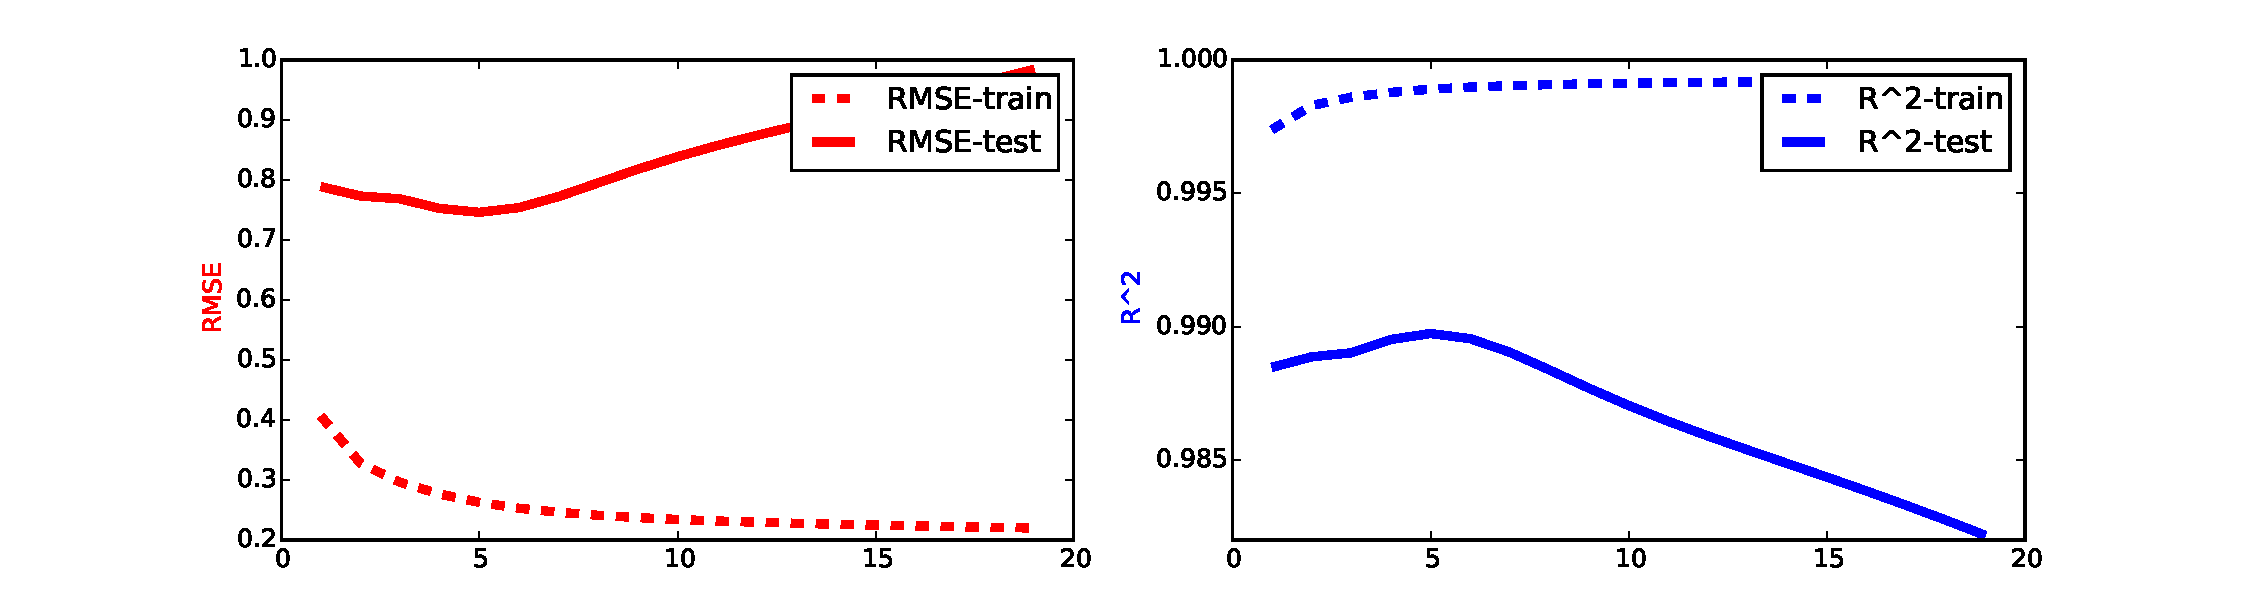
\includegraphics{guide-1.pdf}


\section{Visualizing MCMC Traces}
\label{guide:visualizing-mcmc-traces}
Our MCMC implementation samples model and hyper parameter and every iteration
and calculates a running mean of the predictions. MCMC traces can be used to
evaluate the convergence and mixing behaviour of the chains. The follwing example
demonstrates how to calculate statistics for predictions, hyper parameter and
model parameter efficiently using the \emph{warm\_start} option.

\begin{Verbatim}[commandchars=\\\{\}]
\PYG{k+kn}{import} \PYG{n+nn}{numpy} \PYG{k+kn}{as} \PYG{n+nn}{np}
\PYG{k+kn}{from} \PYG{n+nn}{sklearn.metrics} \PYG{k+kn}{import} \PYG{n}{mean\PYGZus{}squared\PYGZus{}error}
\PYG{k+kn}{from} \PYG{n+nn}{sklearn.cross\PYGZus{}validation} \PYG{k+kn}{import} \PYG{n}{train\PYGZus{}test\PYGZus{}split}

\PYG{k+kn}{from} \PYG{n+nn}{fastFM.datasets} \PYG{k+kn}{import} \PYG{n}{make\PYGZus{}user\PYGZus{}item\PYGZus{}regression}
\PYG{k+kn}{from} \PYG{n+nn}{fastFM} \PYG{k+kn}{import} \PYG{n}{mcmc}

\PYG{n}{n\PYGZus{}iter} \PYG{o}{=} \PYG{l+m+mi}{100}
\PYG{n}{step\PYGZus{}size} \PYG{o}{=} \PYG{l+m+mi}{10}
\PYG{n}{seed} \PYG{o}{=} \PYG{l+m+mi}{123}
\PYG{n}{rank} \PYG{o}{=} \PYG{l+m+mi}{3}

\PYG{n}{X}\PYG{p}{,} \PYG{n}{y}\PYG{p}{,} \PYG{n}{coef} \PYG{o}{=} \PYG{n}{make\PYGZus{}user\PYGZus{}item\PYGZus{}regression}\PYG{p}{(}\PYG{n}{label\PYGZus{}stdev}\PYG{o}{=}\PYG{o}{.}\PYG{l+m+mi}{4}\PYG{p}{)}
\PYG{n}{X\PYGZus{}train}\PYG{p}{,} \PYG{n}{X\PYGZus{}test}\PYG{p}{,} \PYG{n}{y\PYGZus{}train}\PYG{p}{,} \PYG{n}{y\PYGZus{}test} \PYG{o}{=} \PYG{n}{train\PYGZus{}test\PYGZus{}split}\PYG{p}{(}
    \PYG{n}{X}\PYG{p}{,} \PYG{n}{y}\PYG{p}{,} \PYG{n}{test\PYGZus{}size}\PYG{o}{=}\PYG{l+m+mf}{0.33}\PYG{p}{)}

\PYG{n}{fm} \PYG{o}{=} \PYG{n}{mcmc}\PYG{o}{.}\PYG{n}{FMRegression}\PYG{p}{(}\PYG{n}{n\PYGZus{}iter}\PYG{o}{=}\PYG{l+m+mi}{0}\PYG{p}{,} \PYG{n}{rank}\PYG{o}{=}\PYG{n}{rank}\PYG{p}{,} \PYG{n}{random\PYGZus{}state}\PYG{o}{=}\PYG{n}{seed}\PYG{p}{)}
\PYG{c}{\PYGZsh{} Allocates and initalizes the model and hyper parameter.}
\PYG{n}{fm}\PYG{o}{.}\PYG{n}{fit\PYGZus{}predict}\PYG{p}{(}\PYG{n}{X\PYGZus{}train}\PYG{p}{,} \PYG{n}{y\PYGZus{}train}\PYG{p}{,} \PYG{n}{X\PYGZus{}test}\PYG{p}{)}

\PYG{n}{rmse\PYGZus{}test} \PYG{o}{=} \PYG{p}{[}\PYG{p}{]}
\PYG{n}{rmse\PYGZus{}new} \PYG{o}{=} \PYG{p}{[}\PYG{p}{]}
\PYG{n}{hyper\PYGZus{}param} \PYG{o}{=} \PYG{n}{np}\PYG{o}{.}\PYG{n}{zeros}\PYG{p}{(}\PYG{p}{(}\PYG{n}{n\PYGZus{}iter} \PYG{o}{\PYGZhy{}}\PYG{l+m+mi}{1}\PYG{p}{,} \PYG{l+m+mi}{3} \PYG{o}{+} \PYG{l+m+mi}{2} \PYG{o}{*} \PYG{n}{rank}\PYG{p}{)}\PYG{p}{,} \PYG{n}{dtype}\PYG{o}{=}\PYG{n}{np}\PYG{o}{.}\PYG{n}{float64}\PYG{p}{)}
\PYG{k}{for} \PYG{n}{nr}\PYG{p}{,} \PYG{n}{i} \PYG{o+ow}{in} \PYG{n+nb}{enumerate}\PYG{p}{(}\PYG{n+nb}{range}\PYG{p}{(}\PYG{l+m+mi}{1}\PYG{p}{,} \PYG{n}{n\PYGZus{}iter}\PYG{p}{)}\PYG{p}{)}\PYG{p}{:}
    \PYG{n}{fm}\PYG{o}{.}\PYG{n}{random\PYGZus{}state} \PYG{o}{=} \PYG{n}{i} \PYG{o}{*} \PYG{n}{seed}
    \PYG{n}{y\PYGZus{}pred} \PYG{o}{=} \PYG{n}{fm}\PYG{o}{.}\PYG{n}{fit\PYGZus{}predict}\PYG{p}{(}\PYG{n}{X\PYGZus{}train}\PYG{p}{,} \PYG{n}{y\PYGZus{}train}\PYG{p}{,} \PYG{n}{X\PYGZus{}test}\PYG{p}{,} \PYG{n}{n\PYGZus{}more\PYGZus{}iter}\PYG{o}{=}\PYG{n}{step\PYGZus{}size}\PYG{p}{)}
    \PYG{n}{rmse\PYGZus{}test}\PYG{o}{.}\PYG{n}{append}\PYG{p}{(}\PYG{n}{np}\PYG{o}{.}\PYG{n}{sqrt}\PYG{p}{(}\PYG{n}{mean\PYGZus{}squared\PYGZus{}error}\PYG{p}{(}\PYG{n}{y\PYGZus{}pred}\PYG{p}{,} \PYG{n}{y\PYGZus{}test}\PYG{p}{)}\PYG{p}{)}\PYG{p}{)}
    \PYG{n}{hyper\PYGZus{}param}\PYG{p}{[}\PYG{n}{nr}\PYG{p}{,} \PYG{p}{:}\PYG{p}{]} \PYG{o}{=} \PYG{n}{fm}\PYG{o}{.}\PYG{n}{hyper\PYGZus{}param\PYGZus{}}

\PYG{n}{values} \PYG{o}{=} \PYG{n}{np}\PYG{o}{.}\PYG{n}{arange}\PYG{p}{(}\PYG{l+m+mi}{1}\PYG{p}{,} \PYG{n}{n\PYGZus{}iter}\PYG{p}{)}
\PYG{n}{x} \PYG{o}{=} \PYG{n}{values} \PYG{o}{*} \PYG{n}{step\PYGZus{}size}
\PYG{n}{burn\PYGZus{}in} \PYG{o}{=} \PYG{l+m+mi}{5}
\PYG{n}{x} \PYG{o}{=} \PYG{n}{x}\PYG{p}{[}\PYG{n}{burn\PYGZus{}in}\PYG{p}{:}\PYG{p}{]}

\PYG{k+kn}{from} \PYG{n+nn}{matplotlib} \PYG{k+kn}{import} \PYG{n}{pyplot} \PYG{k}{as} \PYG{n}{plt}
\PYG{n}{fig}\PYG{p}{,} \PYG{n}{axes} \PYG{o}{=} \PYG{n}{plt}\PYG{o}{.}\PYG{n}{subplots}\PYG{p}{(}\PYG{n}{nrows}\PYG{o}{=}\PYG{l+m+mi}{2}\PYG{p}{,} \PYG{n}{ncols}\PYG{o}{=}\PYG{l+m+mi}{2}\PYG{p}{,} \PYG{n}{sharex}\PYG{o}{=}\PYG{n+nb+bp}{True}\PYG{p}{,} \PYG{n}{figsize}\PYG{o}{=}\PYG{p}{(}\PYG{l+m+mi}{15}\PYG{p}{,} \PYG{l+m+mi}{8}\PYG{p}{)}\PYG{p}{)}

\PYG{n}{axes}\PYG{p}{[}\PYG{l+m+mi}{0}\PYG{p}{,} \PYG{l+m+mi}{0}\PYG{p}{]}\PYG{o}{.}\PYG{n}{plot}\PYG{p}{(}\PYG{n}{x}\PYG{p}{,} \PYG{n}{rmse\PYGZus{}test}\PYG{p}{[}\PYG{n}{burn\PYGZus{}in}\PYG{p}{:}\PYG{p}{]}\PYG{p}{,} \PYG{n}{label}\PYG{o}{=}\PYG{l+s}{\PYGZsq{}}\PYG{l+s}{test rmse}\PYG{l+s}{\PYGZsq{}}\PYG{p}{,} \PYG{n}{color}\PYG{o}{=}\PYG{l+s}{\PYGZdq{}}\PYG{l+s}{r}\PYG{l+s}{\PYGZdq{}}\PYG{p}{)}
\PYG{n}{axes}\PYG{p}{[}\PYG{l+m+mi}{0}\PYG{p}{,} \PYG{l+m+mi}{0}\PYG{p}{]}\PYG{o}{.}\PYG{n}{legend}\PYG{p}{(}\PYG{p}{)}
\PYG{n}{axes}\PYG{p}{[}\PYG{l+m+mi}{0}\PYG{p}{,} \PYG{l+m+mi}{1}\PYG{p}{]}\PYG{o}{.}\PYG{n}{plot}\PYG{p}{(}\PYG{n}{x}\PYG{p}{,} \PYG{n}{hyper\PYGZus{}param}\PYG{p}{[}\PYG{n}{burn\PYGZus{}in}\PYG{p}{:}\PYG{p}{,}\PYG{l+m+mi}{0}\PYG{p}{]}\PYG{p}{,} \PYG{n}{label}\PYG{o}{=}\PYG{l+s}{\PYGZsq{}}\PYG{l+s}{alpha}\PYG{l+s}{\PYGZsq{}}\PYG{p}{,} \PYG{n}{color}\PYG{o}{=}\PYG{l+s}{\PYGZdq{}}\PYG{l+s}{b}\PYG{l+s}{\PYGZdq{}}\PYG{p}{)}
\PYG{n}{axes}\PYG{p}{[}\PYG{l+m+mi}{0}\PYG{p}{,} \PYG{l+m+mi}{1}\PYG{p}{]}\PYG{o}{.}\PYG{n}{legend}\PYG{p}{(}\PYG{p}{)}
\PYG{n}{axes}\PYG{p}{[}\PYG{l+m+mi}{1}\PYG{p}{,} \PYG{l+m+mi}{0}\PYG{p}{]}\PYG{o}{.}\PYG{n}{plot}\PYG{p}{(}\PYG{n}{x}\PYG{p}{,} \PYG{n}{hyper\PYGZus{}param}\PYG{p}{[}\PYG{n}{burn\PYGZus{}in}\PYG{p}{:}\PYG{p}{,}\PYG{l+m+mi}{1}\PYG{p}{]}\PYG{p}{,} \PYG{n}{label}\PYG{o}{=}\PYG{l+s}{\PYGZsq{}}\PYG{l+s}{lambda\PYGZus{}w}\PYG{l+s}{\PYGZsq{}}\PYG{p}{,} \PYG{n}{color}\PYG{o}{=}\PYG{l+s}{\PYGZdq{}}\PYG{l+s}{g}\PYG{l+s}{\PYGZdq{}}\PYG{p}{)}
\PYG{n}{axes}\PYG{p}{[}\PYG{l+m+mi}{1}\PYG{p}{,} \PYG{l+m+mi}{0}\PYG{p}{]}\PYG{o}{.}\PYG{n}{legend}\PYG{p}{(}\PYG{p}{)}
\PYG{n}{axes}\PYG{p}{[}\PYG{l+m+mi}{1}\PYG{p}{,} \PYG{l+m+mi}{1}\PYG{p}{]}\PYG{o}{.}\PYG{n}{plot}\PYG{p}{(}\PYG{n}{x}\PYG{p}{,} \PYG{n}{hyper\PYGZus{}param}\PYG{p}{[}\PYG{n}{burn\PYGZus{}in}\PYG{p}{:}\PYG{p}{,}\PYG{l+m+mi}{3}\PYG{p}{]}\PYG{p}{,} \PYG{n}{label}\PYG{o}{=}\PYG{l+s}{\PYGZsq{}}\PYG{l+s}{mu\PYGZus{}w}\PYG{l+s}{\PYGZsq{}}\PYG{p}{,} \PYG{n}{color}\PYG{o}{=}\PYG{l+s}{\PYGZdq{}}\PYG{l+s}{g}\PYG{l+s}{\PYGZdq{}}\PYG{p}{)}
\PYG{n}{axes}\PYG{p}{[}\PYG{l+m+mi}{1}\PYG{p}{,} \PYG{l+m+mi}{1}\PYG{p}{]}\PYG{o}{.}\PYG{n}{legend}\PYG{p}{(}\PYG{p}{)}
\end{Verbatim}

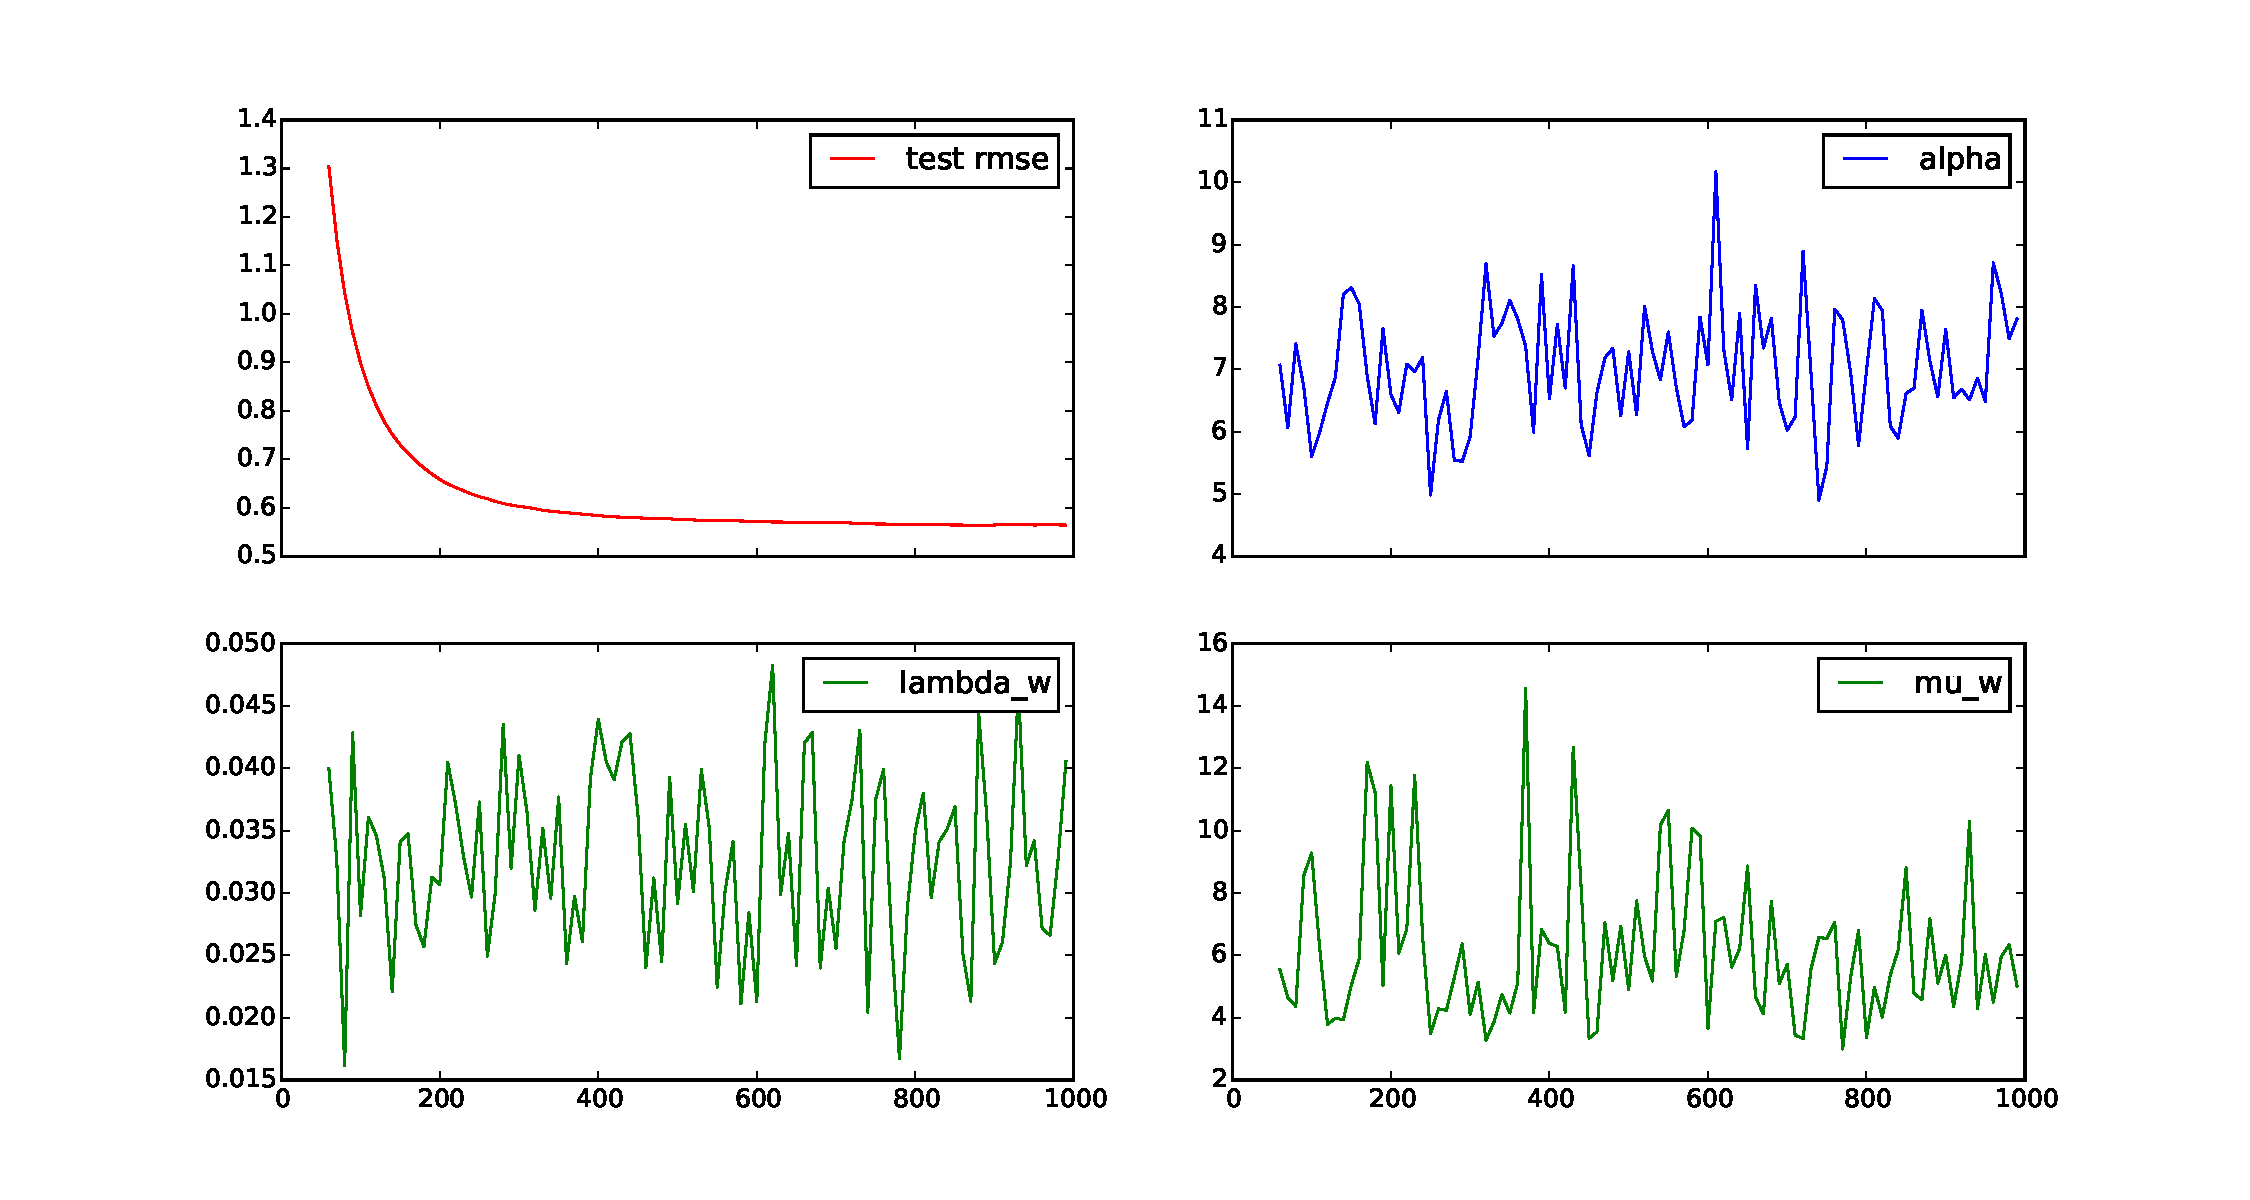
\includegraphics{guide-2.pdf}


\chapter{The fastFM API reference}
\label{api:the-fastfm-api-reference}\label{api::doc}

\section{The MCMC module}
\label{api:the-mcmc-module}\label{api:module-fastFM.mcmc}\index{fastFM.mcmc (module)}\index{FMClassification (class in fastFM.mcmc)}

\begin{fulllineitems}
\phantomsection\label{api:fastFM.mcmc.FMClassification}\pysiglinewithargsret{\strong{class }\code{fastFM.mcmc.}\bfcode{FMClassification}}{\emph{n\_iter=100}, \emph{init\_stdev=0.1}, \emph{rank=8}, \emph{random\_state=123}, \emph{copy\_X=True}}{}
Factorization Machine Classification with a MCMC solver.
\begin{quote}\begin{description}
\item[{Parameters}] \leavevmode\begin{itemize}
\item {} 
\textbf{\texttt{n\_iter}} (\emph{int, optional}) -- The number of samples for the MCMC sampler, number or iterations over
the training set for ALS and number of steps for SGD.

\item {} 
\textbf{\texttt{init\_stdev}} (\emph{float, optional}) -- Sets the stdev  for the initialization of the parameter

\item {} 
\textbf{\texttt{random\_state}} (\emph{int, optional}) -- The seed of the pseudo random number generator that
initializes the parameters and mcmc chain.

\item {} 
\textbf{\texttt{rank}} (\emph{int}) -- The rank of the factorization used for the second order interactions.

\end{itemize}

\end{description}\end{quote}
\index{w0\_ (fastFM.mcmc.FMClassification attribute)}

\begin{fulllineitems}
\phantomsection\label{api:fastFM.mcmc.FMClassification.w0_}\pysigline{\bfcode{w0\_}}
\emph{float}

bias term

\end{fulllineitems}

\index{w\_ (fastFM.mcmc.FMClassification attribute)}

\begin{fulllineitems}
\phantomsection\label{api:fastFM.mcmc.FMClassification.w_}\pysigline{\bfcode{w\_}}
\emph{float \textbar{} array, shape = (n\_features)}

Coefficients for linear combination.

\end{fulllineitems}

\index{V\_ (fastFM.mcmc.FMClassification attribute)}

\begin{fulllineitems}
\phantomsection\label{api:fastFM.mcmc.FMClassification.V_}\pysigline{\bfcode{V\_}}
\emph{float \textbar{} array, shape = (rank\_pair, n\_features)}

Coefficients of second order factor matrix.

\end{fulllineitems}

\index{fit\_predict() (fastFM.mcmc.FMClassification method)}

\begin{fulllineitems}
\phantomsection\label{api:fastFM.mcmc.FMClassification.fit_predict}\pysiglinewithargsret{\bfcode{fit\_predict}}{\emph{X\_train}, \emph{y\_train}, \emph{X\_test}}{}
Return average class probabilities of posterior estimates of the
test samples.
Use only with MCMC!
\begin{quote}\begin{description}
\item[{Parameters}] \leavevmode\begin{itemize}
\item {} 
\textbf{\texttt{X\_train}} (\emph{scipy.sparse.csc\_matrix, (n\_samples, n\_features)}) -- 

\item {} 
\textbf{\texttt{y\_train}} (\emph{array, shape (n\_samples)}) -- the targets have to be encodes as \{-1, 1\}.

\item {} 
\textbf{\texttt{X\_test}} (\emph{scipy.sparse.csc\_matrix, (n\_test\_samples, n\_features)}) -- 

\end{itemize}

\item[{Returns}] \leavevmode
\textbf{y\_pred} --
Returns predicted class labels.

\item[{Return type}] \leavevmode
array, shape (n\_test\_samples)

\end{description}\end{quote}

\end{fulllineitems}

\index{fit\_predict\_proba() (fastFM.mcmc.FMClassification method)}

\begin{fulllineitems}
\phantomsection\label{api:fastFM.mcmc.FMClassification.fit_predict_proba}\pysiglinewithargsret{\bfcode{fit\_predict\_proba}}{\emph{X\_train}, \emph{y\_train}, \emph{X\_test}}{}
Return average class probabilities of posterior estimates of the
test samples.
Use only with MCMC!
\begin{quote}\begin{description}
\item[{Parameters}] \leavevmode\begin{itemize}
\item {} 
\textbf{\texttt{X\_train}} (\emph{scipy.sparse.csc\_matrix, (n\_samples, n\_features)}) -- 

\item {} 
\textbf{\texttt{y\_train}} (\emph{array, shape (n\_samples)}) -- the targets have to be encodes as \{-1, 1\}.

\item {} 
\textbf{\texttt{X\_test}} (\emph{scipy.sparse.csc\_matrix, (n\_test\_samples, n\_features)}) -- 

\end{itemize}

\item[{Returns}] \leavevmode
\textbf{y\_pred} --
Returns probability estimates for the class with lowest
classification label.

\item[{Return type}] \leavevmode
array, shape (n\_test\_samples)

\end{description}\end{quote}

\end{fulllineitems}


\end{fulllineitems}

\index{FMRegression (class in fastFM.mcmc)}

\begin{fulllineitems}
\phantomsection\label{api:fastFM.mcmc.FMRegression}\pysiglinewithargsret{\strong{class }\code{fastFM.mcmc.}\bfcode{FMRegression}}{\emph{n\_iter=100}, \emph{init\_stdev=0.1}, \emph{rank=8}, \emph{random\_state=123}, \emph{copy\_X=True}}{}
Factorization Machine Regression with a MCMC solver.
\begin{quote}\begin{description}
\item[{Parameters}] \leavevmode\begin{itemize}
\item {} 
\textbf{\texttt{n\_iter}} (\emph{int, optional}) -- The number of samples for the MCMC sampler, number or iterations over
the training set for ALS and number of steps for SGD.

\item {} 
\textbf{\texttt{init\_stdev}} (\emph{float, optional}) -- Sets the stdev  for the initialization of the parameter

\item {} 
\textbf{\texttt{random\_state}} (\emph{int, optional}) -- The seed of the pseudo random number generator that
initializes the parameters and mcmc chain.

\item {} 
\textbf{\texttt{rank}} (\emph{int}) -- The rank of the factorization used for the second order interactions.

\end{itemize}

\end{description}\end{quote}
\index{w0\_ (fastFM.mcmc.FMRegression attribute)}

\begin{fulllineitems}
\phantomsection\label{api:fastFM.mcmc.FMRegression.w0_}\pysigline{\bfcode{w0\_}}
\emph{float}

bias term

\end{fulllineitems}

\index{w\_ (fastFM.mcmc.FMRegression attribute)}

\begin{fulllineitems}
\phantomsection\label{api:fastFM.mcmc.FMRegression.w_}\pysigline{\bfcode{w\_}}
\emph{float \textbar{} array, shape = (n\_features)}

Coefficients for linear combination.

\end{fulllineitems}

\index{V\_ (fastFM.mcmc.FMRegression attribute)}

\begin{fulllineitems}
\phantomsection\label{api:fastFM.mcmc.FMRegression.V_}\pysigline{\bfcode{V\_}}
\emph{float \textbar{} array, shape = (rank\_pair, n\_features)}

Coefficients of second order factor matrix.

\end{fulllineitems}

\index{fit\_predict() (fastFM.mcmc.FMRegression method)}

\begin{fulllineitems}
\phantomsection\label{api:fastFM.mcmc.FMRegression.fit_predict}\pysiglinewithargsret{\bfcode{fit\_predict}}{\emph{X\_train}, \emph{y\_train}, \emph{X\_test}, \emph{n\_more\_iter=0}}{}
Return average of posterior estimates of the test samples.
\begin{quote}\begin{description}
\item[{Parameters}] \leavevmode\begin{itemize}
\item {} 
\textbf{\texttt{X\_train}} (\emph{scipy.sparse.csc\_matrix, (n\_samples, n\_features)}) -- 

\item {} 
\textbf{\texttt{y\_train}} (\emph{array, shape (n\_samples)}) -- 

\item {} 
\textbf{\texttt{X\_test}} (\emph{scipy.sparse.csc\_matrix, (n\_test\_samples, n\_features)}) -- 

\item {} 
\textbf{\texttt{n\_more\_iter}} (\emph{int}) -- Number of iterations to continue from the current Coefficients.

\end{itemize}

\item[{Returns}] \leavevmode
\textbf{T}

\item[{Return type}] \leavevmode
array, shape (n\_test\_samples)

\end{description}\end{quote}

\end{fulllineitems}


\end{fulllineitems}



\section{The ALS module}
\label{api:the-als-module}\label{api:module-fastFM.als}\index{fastFM.als (module)}\index{FMClassification (class in fastFM.als)}

\begin{fulllineitems}
\phantomsection\label{api:fastFM.als.FMClassification}\pysiglinewithargsret{\strong{class }\code{fastFM.als.}\bfcode{FMClassification}}{\emph{n\_iter=100}, \emph{init\_stdev=0.1}, \emph{rank=8}, \emph{random\_state=123}, \emph{l2\_reg\_w=0}, \emph{l2\_reg\_V=0}, \emph{l2\_reg=0}}{}
Factorization Machine Classification trained with a ALS
(coordinate descent)
solver.
\begin{quote}\begin{description}
\item[{Parameters}] \leavevmode\begin{itemize}
\item {} 
\textbf{\texttt{n\_iter}} (\emph{int, optional}) -- The number of samples for the MCMC sampler, number or iterations over
the training set for ALS and number of steps for SGD.

\item {} 
\textbf{\texttt{init\_stdev}} (\emph{float, optional}) -- Sets the stdev  for the initialization of the parameter

\item {} 
\textbf{\texttt{random\_state}} (\emph{int, optional}) -- The seed of the pseudo random number generator that
initializes the parameters and mcmc chain.

\item {} 
\textbf{\texttt{rank}} (\emph{int}) -- The rank of the factorization used for the second order interactions.

\item {} 
\textbf{\texttt{l2\_reg\_w}} (\emph{float}) -- L2 penalty weight for pairwise coefficients.

\item {} 
\textbf{\texttt{l2\_reg\_V}} (\emph{float}) -- L2 penalty weight for linear coefficients.

\item {} 
\textbf{\texttt{l2\_reg}} (\emph{float}) -- L2 penalty weight for all coefficients (default=0).

\item {} 
\textbf{\texttt{Attributes}} -- 

\item {} 
\textbf{\texttt{-{-}-{-}-{-}-{-}-}} -- 

\item {} 
\textbf{\texttt{w0}} (\emph{float}) -- bias term

\item {} 
\textbf{\texttt{w}} (\emph{float \textbar{} array, shape = (n\_features)}) -- Coefficients for linear combination.

\item {} 
\textbf{\texttt{V}} (\emph{float \textbar{} array, shape = (rank\_pair, n\_features)}) -- Coefficients of second order factor matrix.

\end{itemize}

\end{description}\end{quote}
\index{fit() (fastFM.als.FMClassification method)}

\begin{fulllineitems}
\phantomsection\label{api:fastFM.als.FMClassification.fit}\pysiglinewithargsret{\bfcode{fit}}{\emph{X\_train}, \emph{y\_train}}{}
Fit model with specified loss.
\begin{quote}\begin{description}
\item[{Parameters}] \leavevmode\begin{itemize}
\item {} 
\textbf{\texttt{X}} (\emph{scipy.sparse.csc\_matrix, (n\_samples, n\_features)}) -- 

\item {} 
\textbf{\texttt{y}} (\emph{float \textbar{} ndarray, shape = (n\_samples, )}) -- the targets have to be encodes as \{-1, 1\}.

\end{itemize}

\end{description}\end{quote}

\end{fulllineitems}


\end{fulllineitems}

\index{FMRegression (class in fastFM.als)}

\begin{fulllineitems}
\phantomsection\label{api:fastFM.als.FMRegression}\pysiglinewithargsret{\strong{class }\code{fastFM.als.}\bfcode{FMRegression}}{\emph{n\_iter=100}, \emph{init\_stdev=0.1}, \emph{rank=8}, \emph{random\_state=123}, \emph{l2\_reg\_w=0}, \emph{l2\_reg\_V=0}, \emph{l2\_reg=0}}{}
Factorization Machine Regression trained with a als (coordinate descent)
solver.
\begin{quote}\begin{description}
\item[{Parameters}] \leavevmode\begin{itemize}
\item {} 
\textbf{\texttt{n\_iter}} (\emph{int, optional}) -- The number of samples for the MCMC sampler, number or iterations over
the training set for ALS and number of steps for SGD.

\item {} 
\textbf{\texttt{init\_stdev}} (\emph{float, optional}) -- Sets the stdev for the initialization of the parameter

\item {} 
\textbf{\texttt{random\_state}} (\emph{int, optional}) -- The seed of the pseudo random number generator that
initializes the parameters and mcmc chain.

\item {} 
\textbf{\texttt{rank}} (\emph{int}) -- The rank of the factorization used for the second order interactions.

\item {} 
\textbf{\texttt{l2\_reg\_w}} (\emph{float}) -- L2 penalty weight for pairwise coefficients.

\item {} 
\textbf{\texttt{l2\_reg\_V}} (\emph{float}) -- L2 penalty weight for linear coefficients.

\item {} 
\textbf{\texttt{l2\_reg}} (\emph{float}) -- L2 penalty weight for all coefficients (default=0).

\item {} 
\textbf{\texttt{Attributes}} -- 

\item {} 
\textbf{\texttt{-{-}-{-}-{-}-{-}-}} -- 

\item {} 
\textbf{\texttt{w0}} (\emph{float}) -- bias term

\item {} 
\textbf{\texttt{w}} (\emph{float \textbar{} array, shape = (n\_features)}) -- Coefficients for linear combination.

\item {} 
\textbf{\texttt{V}} (\emph{float \textbar{} array, shape = (rank\_pair, n\_features)}) -- Coefficients of second order factor matrix.

\end{itemize}

\end{description}\end{quote}
\index{fit() (fastFM.als.FMRegression method)}

\begin{fulllineitems}
\phantomsection\label{api:fastFM.als.FMRegression.fit}\pysiglinewithargsret{\bfcode{fit}}{\emph{X\_train}, \emph{y\_train}, \emph{n\_more\_iter=0}}{}
Fit model with specified loss.
\begin{quote}\begin{description}
\item[{Parameters}] \leavevmode\begin{itemize}
\item {} 
\textbf{\texttt{X}} (\emph{scipy.sparse.csc\_matrix, (n\_samples, n\_features)}) -- 

\item {} 
\textbf{\texttt{y}} (\emph{float \textbar{} ndarray, shape = (n\_samples, )}) -- 

\item {} 
\textbf{\texttt{n\_more\_iter}} (\emph{int}) -- Number of iterations to continue from the current Coefficients.

\end{itemize}

\end{description}\end{quote}

\end{fulllineitems}


\end{fulllineitems}



\section{The SGD module}
\label{api:module-fastFM.sgd}\label{api:the-sgd-module}\index{fastFM.sgd (module)}\index{FMClassification (class in fastFM.sgd)}

\begin{fulllineitems}
\phantomsection\label{api:fastFM.sgd.FMClassification}\pysiglinewithargsret{\strong{class }\code{fastFM.sgd.}\bfcode{FMClassification}}{\emph{n\_iter=100}, \emph{init\_stdev=0.1}, \emph{rank=8}, \emph{random\_state=123}, \emph{l2\_reg\_w=0}, \emph{l2\_reg\_V=0}, \emph{l2\_reg=0}, \emph{step\_size=0.1}}{}
Factorization Machine Classification trained with a stochastic gradient
descent solver.
\begin{quote}\begin{description}
\item[{Parameters}] \leavevmode\begin{itemize}
\item {} 
\textbf{\texttt{n\_iter}} (\emph{int, optional}) -- The number of interations of individual samples .

\item {} 
\textbf{\texttt{init\_std}} (\emph{float, optional}) -- Sets the stdev for the initialization of the parameter

\item {} 
\textbf{\texttt{random\_state}} (\emph{int, optional}) -- The seed of the pseudo random number generator that
initializes the parameters and mcmc chain.

\item {} 
\textbf{\texttt{rank}} (\emph{int}) -- The rank of the factorization used for the second order interactions.

\item {} 
\textbf{\texttt{l2\_reg\_w}} (\emph{float}) -- L2 penalty weight for pairwise coefficients.

\item {} 
\textbf{\texttt{l2\_reg\_V}} (\emph{float}) -- L2 penalty weight for linear coefficients.

\item {} 
\textbf{\texttt{l2\_reg}} (\emph{float}) -- L2 penalty weight for all coefficients (default=0).

\item {} 
\textbf{\texttt{step\_size}} (\emph{float}) -- Stepsize for the SGD solver, the solver uses a fixed step size and
might require a tunning of the number of iterations \emph{n\_iter}.

\item {} 
\textbf{\texttt{Attributes}} -- 

\item {} 
\textbf{\texttt{-{-}-{-}-{-}-{-}-}} -- 

\item {} 
\textbf{\texttt{w0}} (\emph{float}) -- bias term

\item {} 
\textbf{\texttt{w}} (\emph{float \textbar{} array, shape = (n\_features)}) -- Coefficients for linear combination.

\item {} 
\textbf{\texttt{V}} (\emph{float \textbar{} array, shape = (rank\_pair, n\_features)}) -- Coefficients of second order factor matrix.

\end{itemize}

\end{description}\end{quote}
\index{fit() (fastFM.sgd.FMClassification method)}

\begin{fulllineitems}
\phantomsection\label{api:fastFM.sgd.FMClassification.fit}\pysiglinewithargsret{\bfcode{fit}}{\emph{X}, \emph{y}}{}
Fit model with specified loss.
\begin{quote}\begin{description}
\item[{Parameters}] \leavevmode\begin{itemize}
\item {} 
\textbf{\texttt{X}} (\emph{scipy.sparse.csc\_matrix, (n\_samples, n\_features)}) -- 

\item {} 
\textbf{\texttt{y}} (\emph{float \textbar{} ndarray, shape = (n\_samples, )}) -- the targets have to be encodes as \{-1, 1\}.

\end{itemize}

\end{description}\end{quote}

\end{fulllineitems}


\end{fulllineitems}

\index{FMRegression (class in fastFM.sgd)}

\begin{fulllineitems}
\phantomsection\label{api:fastFM.sgd.FMRegression}\pysiglinewithargsret{\strong{class }\code{fastFM.sgd.}\bfcode{FMRegression}}{\emph{n\_iter=100}, \emph{init\_stdev=0.1}, \emph{rank=8}, \emph{random\_state=123}, \emph{l2\_reg\_w=0}, \emph{l2\_reg\_V=0}, \emph{l2\_reg=0}, \emph{step\_size=0.1}}{}
Factorization Machine Regression trained with a stochastic gradient
descent solver.
\begin{quote}\begin{description}
\item[{Parameters}] \leavevmode\begin{itemize}
\item {} 
\textbf{\texttt{n\_iter}} (\emph{int, optional}) -- The number of interations of individual samples .

\item {} 
\textbf{\texttt{init\_stdev}} (\emph{float, optional}) -- Sets the stdev for the initialization of the parameter

\item {} 
\textbf{\texttt{random\_state}} (\emph{int, optional}) -- The seed of the pseudo random number generator that
initializes the parameters and mcmc chain.

\item {} 
\textbf{\texttt{rank}} (\emph{int}) -- The rank of the factorization used for the second order interactions.

\item {} 
\textbf{\texttt{l2\_reg\_w}} (\emph{float}) -- L2 penalty weight for pairwise coefficients.

\item {} 
\textbf{\texttt{l2\_reg\_V}} (\emph{float}) -- L2 penalty weight for linear coefficients.

\item {} 
\textbf{\texttt{l2\_reg}} (\emph{float}) -- L2 penalty weight for all coefficients (default=0).

\item {} 
\textbf{\texttt{step\_size}} (\emph{float}) -- Stepsize for the SGD solver, the solver uses a fixed step size and
might require a tunning of the number of iterations \emph{n\_iter}.

\item {} 
\textbf{\texttt{Attributes}} -- 

\item {} 
\textbf{\texttt{-{-}-{-}-{-}-{-}-}} -- 

\item {} 
\textbf{\texttt{w0}} (\emph{float}) -- bias term

\item {} 
\textbf{\texttt{w}} (\emph{float \textbar{} array, shape = (n\_features)}) -- Coefficients for linear combination.

\item {} 
\textbf{\texttt{V}} (\emph{float \textbar{} array, shape = (rank\_pair, n\_features)}) -- Coefficients of second order factor matrix.

\end{itemize}

\end{description}\end{quote}
\index{fit() (fastFM.sgd.FMRegression method)}

\begin{fulllineitems}
\phantomsection\label{api:fastFM.sgd.FMRegression.fit}\pysiglinewithargsret{\bfcode{fit}}{\emph{X}, \emph{y}}{}
Fit model with specified loss.
\begin{quote}\begin{description}
\item[{Parameters}] \leavevmode\begin{itemize}
\item {} 
\textbf{\texttt{X}} (\emph{scipy.sparse.csc\_matrix, (n\_samples, n\_features)}) -- 

\item {} 
\textbf{\texttt{y}} (\emph{float \textbar{} ndarray, shape = (n\_samples, )}) -- 

\end{itemize}

\end{description}\end{quote}

\end{fulllineitems}


\end{fulllineitems}



\section{The Ranking module}
\label{api:module-fastFM.bpr}\label{api:the-ranking-module}\index{fastFM.bpr (module)}\index{FMRecommender (class in fastFM.bpr)}

\begin{fulllineitems}
\phantomsection\label{api:fastFM.bpr.FMRecommender}\pysiglinewithargsret{\strong{class }\code{fastFM.bpr.}\bfcode{FMRecommender}}{\emph{n\_iter=100}, \emph{init\_stdev=0.1}, \emph{rank=8}, \emph{random\_state=123}, \emph{l2\_reg\_w=0}, \emph{l2\_reg\_V=0}, \emph{l2\_reg=0}, \emph{step\_size=0.1}}{}
Factorization Machine Recommender with pairwise (BPR) loss solver.
\begin{quote}\begin{description}
\item[{Parameters}] \leavevmode\begin{itemize}
\item {} 
\textbf{\texttt{n\_iter}} (\emph{int, optional}) -- The number of interations of individual samples .

\item {} 
\textbf{\texttt{init\_stdev}} (\emph{float, optional}) -- Sets the stdev for the initialization of the parameter

\item {} 
\textbf{\texttt{random\_state}} (\emph{int, optional}) -- The seed of the pseudo random number generator that
initializes the parameters and mcmc chain.

\item {} 
\textbf{\texttt{rank}} (\emph{int}) -- The rank of the factorization used for the second order interactions.

\item {} 
\textbf{\texttt{l2\_reg\_w}} (\emph{float}) -- L2 penalty weight for pairwise coefficients.

\item {} 
\textbf{\texttt{l2\_reg\_V}} (\emph{float}) -- L2 penalty weight for linear coefficients.

\item {} 
\textbf{\texttt{l2\_reg}} (\emph{float}) -- L2 penalty weight for all coefficients (default=0).

\item {} 
\textbf{\texttt{step\_size}} (\emph{float}) -- Stepsize for the SGD solver, the solver uses a fixed step size and
might require a tunning of the number of iterations \emph{n\_iter}.

\item {} 
\textbf{\texttt{Attributes}} -- 

\item {} 
\textbf{\texttt{-{-}-{-}-{-}-{-}-}} -- 

\item {} 
\textbf{\texttt{w0}} (\emph{float}) -- bias term

\item {} 
\textbf{\texttt{w}} (\emph{float \textbar{} array, shape = (n\_features)}) -- Coefficients for linear combination.

\item {} 
\textbf{\texttt{V}} (\emph{float \textbar{} array, shape = (rank\_pair, n\_features)}) -- Coefficients of second order factor matrix.

\end{itemize}

\end{description}\end{quote}
\index{fit() (fastFM.bpr.FMRecommender method)}

\begin{fulllineitems}
\phantomsection\label{api:fastFM.bpr.FMRecommender.fit}\pysiglinewithargsret{\bfcode{fit}}{\emph{X}, \emph{pairs}}{}
Fit model with specified loss.
\begin{quote}\begin{description}
\item[{Parameters}] \leavevmode\begin{itemize}
\item {} 
\textbf{\texttt{X}} (\emph{scipy.sparse.csc\_matrix, (n\_samples, n\_features)}) -- 

\item {} 
\textbf{\texttt{y}} (\emph{float \textbar{} ndarray, shape = (n\_compares, 2)}) -- Each row \emph{i} defines a pair of samples such that
the first returns a high value then the second
FM(X{[}i,0{]}) \textgreater{} FM(X{[}i, 1{]}).

\end{itemize}

\end{description}\end{quote}

\end{fulllineitems}


\end{fulllineitems}


\begin{thebibliography}{SIGIR2011}
\bibitem[TIST2012]{TIST2012}{\phantomsection\label{tutorial:tist2012} 
Rendle, Steffen. ``Factorization machines with libfm.'' ACM Transactions on Intelligent Systems and Technology (TIST) 3.3 (2012): 57.
}
\bibitem[SIGIR2011]{SIGIR2011}{\phantomsection\label{tutorial:sigir2011} 
Rendle, Steffen, et al. ``Fast context-aware recommendations with factorization machines.'' Proceedings of the 34th international ACM SIGIR conference on Research and development in Information Retrieval. ACM, 2011.
}
\end{thebibliography}


\renewcommand{\indexname}{Python Module Index}
\begin{theindex}
\def\bigletter#1{{\Large\sffamily#1}\nopagebreak\vspace{1mm}}
\bigletter{f}
\item {\texttt{fastFM.als}}, \pageref{api:module-fastFM.als}
\item {\texttt{fastFM.bpr}}, \pageref{api:module-fastFM.bpr}
\item {\texttt{fastFM.mcmc}}, \pageref{api:module-fastFM.mcmc}
\item {\texttt{fastFM.sgd}}, \pageref{api:module-fastFM.sgd}
\end{theindex}

\renewcommand{\indexname}{Index}
\printindex
\end{document}
